\opchapter{تشریح سخت‌افزار}\label{chap5}

همانطور که مشخص است، این پروژه از $3$ بخش \emph{نرم‌افزار}، \emph{سرویس
\lr{API}
	 سرور} و \emph{سخت‌افزار} تشکیل شده‌است، که بخش سخت افزار شامل یک کنترل کنندهٔ از راه دور و قلب پردازشی دزدگیر تشکیل شده است.

در بخش سخت‌افزاری کنترل از راه دور
(\lrm{remote})
از یک ریزپردازندهٔ با معماری \lr{AVR} و سری
\lrm{Atmega32p}
 استفاده شده، که برای سهولت کار در حال حاضر از کتابخانه‌ها و برد آمادهٔ‌ \lr{Arduino} برای راه‌اندازی این بخش استفاده شده.

و در مقابل در سمت سخت‌افزار اصلی پروژه نیز از ریزپردازندهٔ
\lrm{ARM}سری \lrm{STM32f013CBT6} استفاده شده، این بخش مستقیماً
و بدون دخالت هیچ برد توسعه‌ای مورد استفاده قرار گرفته‌است.


\section{\rl{کنترل کنندهٔ} \lr{Remote}}\label{sec1:chap5}

همانطور که گفته شد برای این بخش از برد‌های آمادهٔ \lr{Arduino}
استفاده شده‌است.

\lrm{Arduino Pro Mini} یکی از برد‌های توسعه داده‌شده توسط شرکت \lr{Arduino} است، این برد با هستهٔ \lrm{Atmega32p} شامل مشخصات ذیل است:

\begin{itemize}[nosep]
    \item پردازندهٔ $8$ بیت و فرکانس خارجی $8$ مگاهرتز.
    \item $32$ پایه ورودی و خروجی.
    \item یک \lr{SPI}\LTRfootnote{SPI: Serial Peripheral Interface}.
    \item یک \lr{USART}\LTRfootnote{USART: Universal Synchronous/Asynchronous Receiver Transmitter}.
    \item $6$ خروجی \lr{PWM}\LTRfootnote{PWM: Pulse Width Modulation}.
    \item $2$ وقفهٔ خارجی.
    \item $8$ مبدل آنالوگ به دیجیتال (\lr{ADC}\LTRfootnote{ADC: Analog-to-Digital Converter}).
    \item $32$کیلوبایت فضای \lr{SRAM}\LTRfootnote{SRAM: Static Random Access Memory}.
    \item یک کیلوبایت حافظهٔ \lr{EEPROM}\LTRfootnote{EEPROM: Electrically Erasable Programmable Read-Only Memory}.
\end{itemize}
و دیگر موارد است.
\cite{atmega328p_datasheet}

\begin{figure}[!h]
	\begin{center}
		\includegraphics[width=0.4\textwidth]{images/aTmega328p-pins.pdf}
	\end{center}
	\caption{نمایی از پایه‌های خروجی ریزپردازندهّ \lr{AVR}}
	\label{fig1:sec1:chap1}
\end{figure}

\subsection{ماژول‌های خارجی}\label{subsec1:sec1:chap5}

قطعات استفاده شده شامل یک نمایشگر، فرستنده/گیرندهٔ رادیویی،‌ چند دکمه و خازن هستند.


\subsubsection{فرستندهٔ \lr{RF}}\label{subsubsec2:subsec1:sec1:chap5}

ماژول‌های اضافی مورد استفاده در \lr{remote} شامل فرستندهٔ \lr{RF} مدل \lr{HM-TRP} از شرکت سازندهٔ \lr{HopeRF} است، که طبق مشخصات توضیح داده شده در \lr{datasheet} این محصول، یک ماژول به‌صرفه و مصرف منابع بسیار پایین است، برخی از ویژگی‌های این محصول در ذیل لیست شده:
\cite{hmtrp-datasheet}

\begin{itemize}[nosep]
    \item در اندازهٔ بسیار کوچک $16$ در $20$ در $2$ طراحی شده، و در حالت \lr{DIP} و \lr{SMD} قابل نصب است.
    \item کنترل این ماژول توسط \lr{USART} قابل انجام است و فقط کافی است که داده‌ها به ماژول ارسال شوند.
    \item در این ماژول از مدولاسیون \lr{FSK} و برپایهٔ فرکانس استفاده شده که به نسبت مدولاسیون \lr{ASK} ایمن‌تر است.
    \item ارتباط به صورت نیمه-دوطرفه انجام می‌شود.
    \item مصرف این ماژول بین 40 تا \lr{100mW}قابل تغییر است.
    \item و سرعت انتقال داده نیز از $1.2$\lr{Kbps} تا $115.2$\lr{Kbps} قابل تغییر است.
    \item همچنین طبق ادعای شرکت سازنده، برد فرستندهٔ این ماژول در فضای باز تا حداکثر فاصلهٔ $1.5$ کیلومتر است.
\end{itemize}

در ماژول فوق اتصالات بدین ریز پردازنده بدین صورت میباشند.

\begin{figure}[!h]
	\begin{center}
		\includegraphics[width=0.35\textwidth]{images/hmtrp-connections.pdf}
	\end{center}
	\caption{طریقهٔ اتصال ماژول به ریزپردازنده}
	\label{fig1:sec1:chap1}
\end{figure}

\subsubsection{صفحهٔ نمایش \lr{OLED}}\label{subsubsec3:subsec1:sec1:chap5}

در تعریف
\lr{OLED}\LTRfootnote{Organic Light-Emitting Diode.}
 یک \lr{LED} است که از یک لایهٔ
ترکیب آلی استفاده شده که در اثر یک جریان یا میدان الکتریکی از خود نور ساطع می‌کند.

در این پروژه در سخت‌افزار \lr{remote} برای نمایش اطلاعات خودرو از یک نمایشگر \lr{OLED} از سری
\lrm{ER-OLEDM0.91}
 با اندازهٔ
$128\times32$
  پیکسل استفاده شده‌است.

این نمایشگر دارای ارتباط
\lr{I2C}\LTRfootnote{Inter Integrated Circuit.}
 است و می‌تواند با ولتاژ $3.3$ تا $5.5$ راه‌اندازی شود، همچنین مصرف جریان این ماژول از $23$ تا $27$ میلی آمپر است.

این نمایشگر در دستهٔ
\lr{PMOLED}\LTRfootnote{Active Matrix OLED.}
 قرار می‌گیرد که مصرف بیشتری به نسبت
\lr{AMOLED}\LTRfootnote{Passive Matrix OLED.}
 دارد، اما مصرف نمایشگر‌های \lr{OLED} نسبت نمایشگر‌های \lr{LCD} کمتر هستند.
\cite{OrganicE14:online}

طریقهٔ اتصال پین‌های نمایشگر به
\lr{remote}
به صورت زیر است:

\begin{figure}[!h]
	\begin{center}
		\includegraphics[width=0.35\textwidth]{images/oled-connections.pdf}
	\end{center}
	\caption{طریقهٔ اتصال ماژول \lr{OLED} به پردازنده}
	\label{fig1:sec1:chap5}
\end{figure}

\section{سخت‌افزار اصلی (\lr{Main Board})}\label{sec2:chap5}

سخت‌افزار اصلی شامل ریز پردازندهٔ \lrm{STM32} با معماری \lr{ARM} و از سری \lrm{STM32F103CBT6} است، که مشخصات این ریز پردازنده مطابق ذیل است:

\begin{itemize}[nosep]
    \item دارای سه \lrm{USART}، دو \lrm{SPI}، دو \lrm{I2C}، یک ارتباط \lrm{USB}، یک زمان‌سنج  \lrm{PWM}، و یک ارتباط سخت‌افزاری \lrm{CAN} است.
    \item همچنین دارای $48$ پین (پکیج \lrm{LQFP48}\LTRfootnote{Low-profile Quad Flat Pack 48}).
    \item که $37$ تا از آن‌ها ورودی و خروجی است.
    \item دارای $7$ زمان‌سنج.
    \item $2$ مبدل آنالوگ به دیجیتال سخت‌افزاری (با دقت $12$ بیت).
    \item ولتاژ کاری $2.0$ تا $3.6$.
    \item
    و دمای کاری منفی $40$$\deg$ تا $85$$\deg$ درجهٔ سانتی‌گراد است.
    \item همچنین $64$ کیلوبایت حافظهٔ قابل برنامه‌نویسی \lr{FLASH} و $20$ کیلوبایت حافظهٔ
\lr{SRAM} را داراست.
\end{itemize}

در عکس زیر نیز شمای کلی این ریزپردازنده قابل مشاهده است.

\begin{figure}[!h]
	\begin{center}
		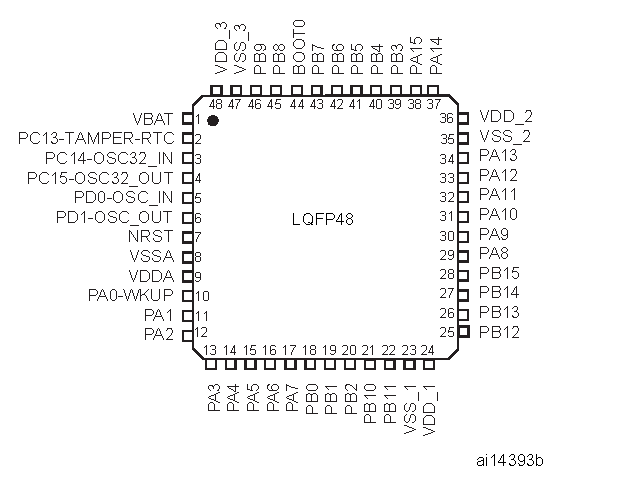
\includegraphics[width=0.6\textwidth]{images/STM32103xx.pdf}
	\end{center}
	\caption{نمایی از پایه‌های خروجی ریزپردازندهّ \lr{STM32F103CBT6}}
	\label{fig1:sec2:chap1}
\end{figure}


دلیل انتخاب این ریزپردازنده قیمت نصب و با امکانات سه برابری نسبت به نسخهٔ
\lrm{ARM}
 هست، همچنین با توجه به تعداد بالای قطعات خارجی نیاز به وجود حداقل $3$
\lrm{USART}
 سخت‌افزاری است، که در این ریزپردازنده فراهم شده است.

\subsection{ماژول‌های خارجی}\label{subsec1:sec2:chap5}

در این بخش از پروژه از ماژول‌های \lr{GPS}، ماژول \lr{GSM}،‌ فرستنده/گیرندهٔ رادیویی،
چند رله، ماسفت و دیگر قطعات استفاده شده است.


\subsubsection{ماژول \lr{GPS}}\label{subsubsec1:subsec1:sec2:chap5}

ماژول \lr{GPS} در این پروژه برای موقعیت یابی استفاده شده است، این ماژول از سری \lrm{neo6mv2} و ساختهٔ شرکت \lr{ublox} است.

ارتباط با این ماژول از طریق \lr{USART} صورت می‌گیرد که در صورت اتصال موفق به ماهواره، به صورت پیاپی و در هر ثانیهٔ اطلاعات مربوط به موقعیت از طریق \lr{USART} به پردازنده ارسال می‌شود.

این اطلاعات شامل موقعیت جغرافیایی، فاصله از سطح دریا، تعداد ماهواره‌های در دسترس، سرعت، زمان در فرمت \lr{UTC} و موارد دیگر است، که در زیر دسته‌های این اطلاعات لیست شده است:

\begin{itemize}[nosep]
    \item \lrm{\$GPGSA}: اطلاعات مربوط به ماهواره‌های فعال.
    \item \lrm{\$GPGSV}: ریز اطلاعات مربوط به ماهوارهٔ \lr{GPS}.
    \item \lrm{\$GPGLL}: اطلاعات جغرافیایی از جمله عرض و طول جغرافیایی.
    \item \lrm{\$GPRMC}: اطلاعات ضروری مانند سرعت، زمان، و شتاب.
    \item \lrm{\$GPVTG}: اطلاعات مربوط به جهت حرکت، و سرعت زمان.
\end{itemize}

در اینجا فقط از اطلاعات در خط \lr{GPGGA} استفاده شده است که خلاصهٔ اطلاعات ضروری \lr{GPS} است، این اطلاعات با مقدار \lr{\$GPGGA} شروع شده و سپس به دنبال آن $14$ فیلد دادهٔ دیگر جدا شده توسط «,» (\lr{comma}) قرار گرفته‌اند، این اطلاعات به ترتیب شامل لیست

\textit{
\hypersetup{linkcolor=gray}
\hyperref[i1:enum1:sec2:chap5]{utc},
\hyperref[i2:enum1:sec2:chap5]{latitude},
\hyperref[i3:enum1:sec2:chap5]{N},
\hyperref[i4:enum1:sec2:chap5]{Longitude},
\hyperref[i5:enum1:sec2:chap5]{W},
\hyperref[i6:enum1:sec2:chap5]{quality-code},
\hyperref[i7:enum1:sec2:chap5]{satellites-num},
\hyperref[i8:enum1:sec2:chap5]{horizontal-dilution},
\hyperref[i9:enum1:sec2:chap5]{altitude},
\hyperref[i10:enum1:sec2:chap5]{M},
\hyperref[i11:enum1:sec2:chap5]{mean-sea-level},
\hyperref[i12:enum1:sec2:chap5]{M},
\hyperref[i13:enum1:sec2:chap5]{last-DGPS-UTC \textbar{} dgps-station-id},
\hyperref[i14:enum1:sec2:chap5]{checksum}
}
است.
\begin{enumerate}[nosep]
    \item \label{i1:enum1:sec2:chap5}\lr{UTC} زمان اتصال به ماهواره و ثابت شدن در میلی‌ثانیه.
    \item \label{i2:enum1:sec2:chap5}\lr{latitude} عرض جغرافیایی.
    \item \label{i3:enum1:sec2:chap5}\lr{N} علامت جهت شما یا جنوب.
    \item \label{i4:enum1:sec2:chap5}\lr{longitude} طول جغرافیایی.
    \item \label{i5:enum1:sec2:chap5}\lr{W} علامت جهت غرب با شرق.
    \item \label{i6:enum1:sec2:chap5}\lr{quality-code} کد ثبات \lr{GPS}: \lrm{0} (نا معتبر)، \lrm{1} (ثبات \lr{GPS}), \lrm{2} (ثبات \lr{DGPS}), \lrm{3}
    (ثبات \lr{PPS}) , \lrm{4} (بی‌درنگ), \lrm{5} (\lr{Float RTK}), \lrm{6} (تقریبی), \lrm{7} (ورودی دستی), \lrm{8}
    (حالت شبیه‌سازی)
    \item \label{i7:enum1:sec2:chap5}\lr{satellites-num} تعداد ماهواره‌های تشخیص داده شده.
    \item \label{i8:enum1:sec2:chap5}\lr{horizontal-dilution} اندازه گیری کیفیت هندسی ماهواره های \lr{GPS} در دید.
    \item \label{i9:enum1:sec2:chap5}\lr{altitude} ارتفاع از سطح دریا.
    \item \label{i10:enum1:sec2:chap5}\lr{M} واحد ارتفاع.
    \item \label{i11:enum1:sec2:chap5}\lr{mean-sea-level} تفاوت ارتفاع بین بیضی مرجع \lr{WGS84} و ژئوئید زمین.
    \item \label{i12:enum1:sec2:chap5}\lr{M} واحد ارتفاع.
    \item \label{i13:enum1:sec2:chap5}\lr{last-DGPS-UTC} --زمان از آخرین بروز رسانی \lr{DGPS. DGPS-station-id -- DGPS station ID number }
    \item \label{i14:enum1:sec2:chap5}*42 -- دادهٔ تشخیص صحت مقدار، همیشه با \lrm{*} شروع می‌شود.
\end{enumerate}

در اینجا اطلاعات در پردازندهٔ \lr{STM32} دریافت شده و مقادیر توسط «,» جدا می‌شوند، سپس به صورت یک ساختار در یک \lr{ring-buffer} ذخیره می‌شوند.

در مقابل این ماژول، ماژول‌های سری \lr{L} از شرکت \lr{Quectel} قرار می‌گیرند که به ظاهر کیفیت بهتری دارند، اما به نسبت قیمت ماژول‌های شرکت \lr{ublox} مقرون به‌صرفه‌تر هستند.
\cite{GPVTG21:online}

\subsubsection{ماژول \lr{SIM800L}}\label{subsubsec2:subsec1:sec2:chap5}

برای ارسال داده‌ها به سمت سرور نیاز به اتصال به اینترنت است که این اتصال به واسطهٔ ماژول‌های سیم‌کارت صورت می گیرد.

از جمله ماژول‌های بیشتر مورد استفاده شده ماژول \lrm{SIM800L} است که ارزان‌ترین ماژول \lr{GSM} از شرکت \lr{SimCom} است، ماژول \lrm{SIM800L} امکان برقراری ارتباط به صورت \lr{2G} را فراهم می‌کند.

این ماژول همچنین قابلیت ارسال و دریافت پیام‌کوتاه، ارسال ایمیل، ایجاد تماس صوتی، ارسال \lr{MMS}، ضبط صوت، ایجاد ارتباط \lr{FTP}، ایجاد درخواست \lr{HTTP} و دیگر موارد را داراست.

تقریباً در اکثر نقاط کشور امکان ارتباط به صورت \lr{2G} فراهم شده‌است، پس یکی به‌صرفه ترین راه‌ها برای اتصال به سرور استفاده از ماژول‌های سیم‌کارت است.

همچنین از راه‌های دیگر ارتباط اینترنتی در نقاط مختلف، می‌‌توان به ارتباط‌های ماهواره‌ای از طریق ماژول‌های \lr{LORA} و \lr{Swarm} از شرکت \lr{Space X} اشاره کرد که راه‌حلی جدید برای اینترنت‌اشیاء در تمامی نقاط است، اما به نسبت هزینه در مقابل \lr{SIM800L} به‌صرفه نیست.

این ماژول از ارتباط \lr{USART} برای ارسال و دریافت داده‌ها به پردازنده استفاده می‌کند، و دستورات به صورت مجموعه‌ای از \lr{AT-Command}ها به ماژول ارسال می شوند.

ماژول‌های \lr{SIM800} دارای پیچیدگی بسیار بالایی هستند و یک محدودهٔ‌ بزرگی از امکانات را در اختیار توسعه‌دهنده قرار می‌دهند، و طبق ادعای شرکت \lr{SimCOM} تمامی قابلیت‌های یک تلفن هوشمند و یا یک کامپیوتر شخصی را به شما می‌دهند.

در ادامهٔ مشخصات ماژول \lr{SIM800L}، این ماژول نیاز به توان ورودی بین $3.4$ تا $4.4$ ولت را نیاز دارد. این ماژول در حالت خواب (\lr{sleep mode}) فقط $0.7$
میلی‌آمپر توان مصرف می‌کند. این ماژول همچنین از $4$ باند فرکانس‌های \lr{GSM} پشتیبانی می‌کند، که توان ارسال آن وابسته به باند فرکانس تنظیم شده است.
همچنین دمای کاری ماژول بین منفی $40$ تا $85$ درجهٔ سانتیگراد است.

ارسال داده‌های \lr{GPRS} نیز می‌تواند تا حداکثر سرعت $85$\lr{Kbps} انجام پذیرد. ماژول از قابلیت‌ \lr{USSD} پشتیبانی می‌کند و همچنین دارای پشتیبانی از نسخه‌های سیم‌کارت $1.8$ تا نسخهٔ $3$ است.

می‌توان برای تقویت ماژول از یک آنتن خارجی استفاده کرد. این ماژول در بخش صورت دارای قابلیت های رفع نویز و رفع اکو نیز است. و دارای قابلیت \lr{Real time} است که همچنین قابل فعال‌سازی است.

اندازهٔ ماژول در \lr{15.8x17.8x2.4mm} است و دارای وزن $1.35$ گرم است.
\cite{sim800}

\paragraph{طریقهٔ اتصال}\label{par1:subsubsec1:subsec1:sec2:chap5}

بر روی ماژول‌های موجود در بازای یک محافظ فلزی برای جلوگیری از آسیب دیدگی و رفع نویز قرار داده شده، که همچنین برای استفادهٔ راحت‌تر عموماً توسط یک مبدل \lr{DIP} به فروش می‌رسند که تا $12$ پین از آن در دسترس است.
پین‌های خروجی ماژول به صورت زیر هستند:

\begin{figure}[!h]
	\begin{center}
		\includegraphics[width=0.3\textwidth]{images/sim800-pins.pdf}
	\end{center}
	\caption{پین‌های خروجی در ماژول \lr{SIM800L}}
	\label{fig1:sec2:chap5}
\end{figure}

\LTRfootnotetext{DTR: Data Ready.}
\LTRfootnotetext{GND: Ground.}
\LTRfootnotetext{MIC: Microphone.}
\LTRfootnotetext{Net: Antena.}
\LTRfootnotetext{RING: Phone Ring.}
\LTRfootnotetext{RST: Reset.}
\LTRfootnotetext{RXD: UART data reciver.}
\LTRfootnotetext{SPK: Speaker.}
\LTRfootnotetext{TXD: UART data transmiter.}

در کنار این توضیحات،‌ استفاده از این ماژول نیازمند کمی دانش اولیه برای راه‌اندازی آن است، که این نکات عبارت‌اند از:

\begin{enumerate}[nosep]
    \item بهتر است ورودی توان ماژول مقدار $4.4$ ولت باشد، هر مقداری بیش‌از این موجب سوختن ماژول خواهد شد. همچنین جریان ورودی مورد نیاز در حالت مناسب باید تا $2$ آمپر باشد.
    \item برای استفاده از مآژول توصیه شده که از ولتاژ $3.3$ برای ورودی \lr{TX}استفاده شود. این کار می تواند با قراردهی یک دیود در بین پایه‌های \lr{TX} و \lr{RX} انجام شود.
    \item برای بررسی فعال بودن یا نبودن ماژول می‌توان پین \lr{Ring} را بررسی کرد، که باید همیشه مقدار آن $4$ ولت باشد.
    \item برای تشخیص راه‌اندازی مجدد شدن ماژول می‌توان گزینه‌های زیر را برررسی کرد،
    در صورت راه‌اندازی مجدد به احتمال زیاد توان کافی به ماژول نمی‌رسد و باید این مشکل رفع گردد:

    \begin{enumerate}[nosep]
        \item نشانگر \lr{LED} وضعیت ماژول به سرعت چشمک زده، متوقف شود و سپس مجدداً به چشمک زدن ادامه پیدا کند. بدین معنی که ماژول در اتصال به شبکه مشکل داشته و توان کافی به ماژول نرسیده، پس ماژول شروع به راه‌اندازی مجدد می‌کند.
        \item اگر مقدار پین \lr{Ring} صفر شد.
        \item در صورت ارسال شدن مقدار نال (\lr{Null}) از طریق \lr{USART}.
        \item مشاهدهٔ مقدار \lrm{SMS\ Ready}یا \lrm{Call\ Ready} بعد از هر دستور.
    \end{enumerate}
    \item ماژول‌های \lr{SIM800} برای اتصال به شبکه نیازمند جریان لحظه‌ای $2$ آمپر هستند،
    که عموماً فراهم کردن تغذیه‌ای با خروجی $2$ آمپر ممکن نیست، برای رفع این مشکل می‌توان از یک خازن $1500$\lr{uF} در بین پایه‌های زمین و $4$ ولت استفاده کرد.
    همچنین استفاده از خازن‌های پلیمری برای اینکار توصیه می‌شوند.
\end{enumerate}


\paragraph{دستورات}\label{par2:subsubsec1:subsec1:sec2:chap5}

برخی از دستورات مهم ماژول به شرح زیر هستند:

\begin{enumerate}[nosep]
    \item \lrm{ATA}: پاسخ تماس.
    \item \lrm{ATZ}: بازنشانی تنظیمات پیشفرض.
    \item \lrm{ATI}: اطلاعات ماژول.
    \item \lrm{ATD+980123456789;}: ایجاد تماس.
    \item \lrm{ATH}:پایان تماس.
    \item \lrm{AT\&F}: تنظیمات کارخانه.
    \item \lrm{AT\&V}: نمایش تنظیمات فعلی.
    \item \lrm{AT\&W}: ذخیرهٔ نمایهٔ فعال.
    \item \lrm{AT+HVOIC}: قطع فقط تماس.
    \item \lrm{AT+CPOWD=1}: خاموش کردن ماژول.
    \item \lrm{AT+CPOWD=0}: خاموش کردن فوری.
    \item \lrm{AT+SJDR=\textless{}n\textgreater{}}: تنظیم تشخیص اختلال.
    \item \lrm{AT+CANT=1,0,10}: فعال‌سازی تشخیص آنتن.
    \item \lrm{AT+CANT=1,1,10}: فعال‌سازی تشخیص آنتن و اطلاع رسانی آن هر $10$
    ثانیه.
    \item \lrm{AT+CROAMING}: حالت رومینگ.
    \item \lrm{AT+CBATCHK=1}: تنظیم ولتاژ پشتیبانی.
    \item \lrm{AT+CPAS}: گزارش وضعیت ماژول.
    \item \lrm{AT+CSQ}: گزارش کیفیت سیگنال.
    \item \lrm{AT+CFUN=1}: تنظیم عملکرد ماژول.
    \item \lrm{AT+CFUN=1,1}: راه‌اندازی مجدد و تنظیم عملکرد کامل ماژول.
    \item \lrm{AT+CCLK?}: ساعت.
    \item \lrm{AT+CBC}: میزان باتری.
    \item \lrm{AT+CSCLK?}: فعال‌سازی حالت آهسته.
    \item \lrm{AT+CSCLK=0}: غیر فعال‌سازی حالت آهسته.
    \item \lrm{AT+CENG}: تغییر به حالت مهندسی.
\end{enumerate}

\paragraph{\lr{GPRS}}\label{par3:subsubsec1:subsec1:sec2:chap5}
\begin{enumerate}[nosep]
    \item \lrm{AT+CGATT=1}: اتصال یا قطع ارتباط \lr{GPRS}.
    \item \lrm{AT+SAPBR=3,1,"Contype","GPRS"}: تنظیم نوع اتصال \lr{GPRS}.
    \item \lrm{AT+SAPBR=3,1,"APN","mtnirancell"}: تنظیم مقدار \lr{APN} اپراتور.
    \item \lrm{AT+SAPBR=1,1}: فعال‌سازی \lr{GPRS}.
    \item \lrm{AT+SAPBR=0,1}: قطع \lr{GPRS}.
    \item \lrm{AT+SAPBR=2,1}: گرفتن مقدار \lr{IP}.
\end{enumerate}

\paragraph{دستورات آمادهٔ پیاپی}\label{par4:subsubsec1:subsec1:sec2:chap5}

در زیر لیستی از دستورات و روال‌ها برای انجام برخی عملیات ضروری‌تر توسط ماژول فراهم شده است.
باید توجه کرد که اجرای دستورات باید به صورت سری و پشت سر هم و با وقفهٔ بسیار کم باشند.
همچنین اجرای هر دستور نیازمند فعال‌سازی دستورات قبل است.

\subparagraph{\rl{راه‌اندازی مجدد}}\label{subpar1:par4:subsubsec1:subsec1:sec2:chap5}
\:\newline\:
\begin{latin}
	\small
	\begin{lstlisting}[language=bash,caption={restarting module}]
        # Airplane mode
        AT+CFUN=0
		# Full function
		AT+CFUN=1
	\end{lstlisting}
\end{latin}

\subparagraph{\rl{فعال‌سازی} \lr{GPRS}}\label{subpar2:par1:subsubsec1:subsec1:sec2:chap5}
\:\newline\:
\begin{latin}
	\small
	\begin{lstlisting}[language=bash,caption={Enable GPRS}]
		# AT+SAPBR=<type>,<cid>[,<param>,<value>]
		# <type>: 0.close 1.open 2.open 3.set parameter
		# Set connection type
		AT+SAPBR=3,1,"Contype","GPRS"
		# Set APN(Access Point Name)
		AT+SAPBR=3,1,"APN","mtnirancell"
		# Enable GPRS, Open bearer
		AT+SAPBR=1,1
		# Query bearer
		AT+SAPBR=2,1
	\end{lstlisting}
\end{latin}

\subparagraph{\rl{غیرفعال‌سازی} \lr{GPRS}}\label{subpar3:par1:subsubsec1:subsec1:sec2:chap5}
\:\newline\:
\begin{latin}
	\small
	\begin{lstlisting}[language=bash,caption={Disabling GPRS}]
		# Disable GPRS
		AT+SAPBR=0,1
	\end{lstlisting}
\end{latin}

\subparagraph{\rl{درخواست} \lr{HTTP}}\label{subpar4:par1:subsubsec1:subsec1:sec2:chap5}
\:\newline\:
درخواست‌های \lr{Http} در ماژول \lr{SIM800} بعد از فعال‌سازی \lr{GPRS} ممکن است، اما احتمال موفقیت ارسال این درخواست نسبت به ایجاد ارتباط خام \lr{TCP} کمتر است،
به این دلیل که تعداد دستورات بیشتر بوده و متأسفانه رابط استفاده از دستورات به هیچ عنوان مناسب نیست، و استفاده از این رابط به شدت مشکل است.

پس در این پروژه مستقیماً درخواست‌ها به صورت درخواست خام \lr{TCP} ارسال شده‌اند.

\begin{latin}
	\small
	\begin{lstlisting}[language=bash,caption={HTTP request}]
		# Initialize
		AT+HTTPINIT

		# Add Http params
		# AT+HTTPPARA=<param name>,<value>
		# AT+HTTPPARA="CID",<profile-id>
		AT+HTTPPARA="CID",1

		# AT+HTTPPARA="URL",<target url>
		AT+HTTPPARA="URL","http://cardian.ir/graphql"

		# Set Http content-type
		# AT+HTTPPARA="CONTENT","<mime types>"
		AT+HTTPPARA="CONTENT","application/json"

		# AT+HTTPDATA=<data size>,<wait in ms>
		AT+HTTPDATA=192,5000

		# Post DATA, if there is a post
		postdata

		# AT+HTTPACTION=<action>
		# <action>:0 GET, 1 POST, 2 HEAD, 3 DELETE
		AT+HTTPACTION=0

		# Read all data
		AT+HTTPREAD

		# Terminate HTTP Service
		AT+HTTPTERM
	\end{lstlisting}
\end{latin}

\subparagraph{\rl{ایجاد ارتباط} \lr{TCP}}\label{subpar5:par1:subsubsec1:subsec1:sec2:chap5}
\:\newline\:
\begin{latin}
	\small
	\begin{lstlisting}[language=bash,caption={TCP connection}]
		# set to single connection
		AT+CIPMUX=0
		# Set default APN
		AT+CSTT="mtnirancell","",""
		# Start wireless connection
		AT+CIICR
		# Get assigned IP address
		AT+CIFSR

		# Close old connections (optional)
		# $ SHUT OK
		AT+CIPSHUT
		# manually read data (optional)
		AT+CIPRXGET=1
		# AT+CIPSTART="<TCP/UDP>","<server>","<port>"
		AT+CIPSTART="TCP","cardian.ir",80
		# Send TCP packet
		# AT+CIPSEND=<data-length>
		AT+CIPSEND=107

		POST /index.html HTTP/1.0\nHOST: cardian.ir\nContent-type: application/json\nContent-length: 13\n{"test":true}\n

		# Close TCP connection
		AT+CIPCLOSE
	\end{lstlisting}
\end{latin}

\emph{\textbf{نکته}: در صورتی که مقدار \lrm{+PDP:\ DEACT\ URC} توسط ماژول گزارش شد به معنی جداسازی و قطع شدن \lrm{GPRS} توسط شبکه است. در این حالت کاربر باید دستور \lrm{AT+CIPSHUT} را برای تغییر زمینهٔ
\lrm{PDP} به حالت اصلی انجام دهد. در غیر این صورت امکان اتصال مجدد \lr{GPRS} به شبکه نیست.}
\cite{sim800}

\section{طراحی شماتیک و فیبر مدار چاپی}\label{sec3:chap5}
برای طراحی شماتیک \footnote{یک نمایش گرافیکی است که از اجزاء مختلف یک مدار الکتریکی و اتصالات بین آن‌ها تشکیل شده‌است.}
 مدار از برنامهٔ
\lr{Altium Designer}\LTRfootnote{\url{https://www.altium.com}}
استفاده شده‌است.

در این پروژه طراحی شماتیک برای بخش‌های مدار اصلی و کنترل انجام شده‌است.

\subsection{برد اصلی}\label{subsec1:sec3:chap5}
طراحی شماتیک مدار اصلی در زیر آمده‌است.
\begin{figure}[!h]
	\begin{center}
		\includegraphics[width=0.8\textwidth]{images/main-hardware-schematic.pdf}
	\end{center}
	\caption{شماتیک مدار اصلی}
	\label{fig1:sec3:chap5}
\end{figure}

\begin{figure}[!h]
	\centering
	\footnotesize
	\begin{subfigure}[t]{0.50\linewidth}
		\centering
		\includegraphics[width=\textwidth]{images/pcb-top-layer.pdf}
		\caption{لایهٔ بالایی}
		\label{subfig1:fig2:sec3:chap5}
	\end{subfigure}
	\begin{subfigure}[t]{0.44\linewidth}
		\centering
		\includegraphics[width=\textwidth]{images/3d-preview.jpg}
		\caption{پیش‌نمایش سه بعدی}
		\label{subfig2:fig2:sec3:chap5}
	\end{subfigure}
	\normalsize
	\label{fig2:sec3:chap5}
	\caption{فیبر مدار چاپی}
\end{figure}

قطعات استفاده شده در شماتیک مطابق لیست زیر است:

\begin{enumerate}[nosep]
	\item \lrm{1x3 Pin Header}.
	\item \lrm{STM32F103CBT6}.
	\item \lrm{SIM800L}.
	\item \lrm{Nano SIM Connector}.
	\item \lrm{NEO-M6-V2 GPS}.
	\item \lrm{HM-TRP 433MHz}.
	\item \lrm{Crystal-XL7KI-111-32M}.
	\item
	\lrm{1206-SMD-Capacitor}:
	\lrm{8pF} ($2$)،
	\lrm{15uf} ($4$).
	\item \lrm{Tantalium Capacitor}.
	\item \lrm{IPEX-MHF1} ($2$).
	\item \lrm{LU-3H Relay} ($6$).
	\item \lrm{SHT20 Temperature Sensor}.
	\item \lrm{1206 SMD LED} ($5$).
	\item \lrm{1206 SMD Resistor}:
	\lrm{10} ($1$)،
	\lrm{1K} ($8$)،
	\lrm{330} ($6$)\footnote{برای استفاده به همراه \lr{LED}ها.}.
	\item \lrm{PHD45N03LTA Mosfet}.
	\item \lrm{3x6 SMD Tacticle Switch}.
	\item \lrm{3.3 Linear Regulator SOT-223}.
\end{enumerate}